%--------------------------------------
\chapter{The MASC Framework}
\label{chap_framework}
%--------------------------------------
\begin{figure*}[!ht]
	\centering
    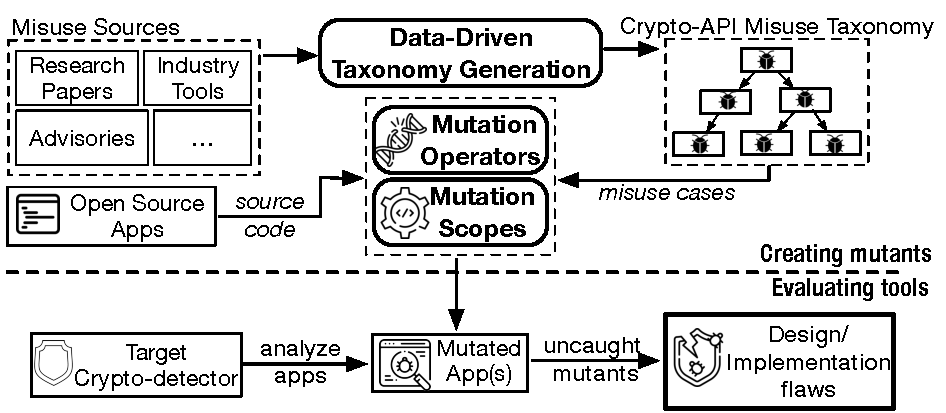
\includegraphics[width=0.96\linewidth]{figures/overview.pdf}
	\vspace{-1.em}
    \caption{\small A basic overview diagram showing how the MASC Framework was designed}
    \label{fig:overview}
	
\end{figure*}
%--------------------------------------
\section{Overview}
\label{ch2:sec:overview}
%--------------------------------------

The original work proposed a framework for Mutation-based Analysis of Static Crypto-misuse detection techniques (or MASC). Figure 2.1 above shows the design of the MASC framework as described in the original work. The framework remains the same and all the ideas from this original framework were intentionally consistent throughout my work as well. Cryptographic libraries contain many sets of API with a variety of potential misuse cases, this resulted in an incredibly large design space. Due to this the original work decided to start MASC by creating a "data-driven taxonomy crypto API misuse." This allows for the misuse cases to be grounded based on what is seen in practice. This both allows for a more focused design space and helps justify the misuses MASC puts into practice. For this extension the taxonomy was expanded to include more cases than the prior work and updated with newer misuses and additional confirmation of previous misuses.

Misuses had to be handled in a way that allowed for some flexibility since misuses can appear in a variety of ways. For example the original paper provides the example of DES can be provided as a variable in Cipher.getInstance(<parameter>) and can also be provided in lowercase. To be able to express both of these without hard coding them as examples MASC is designed by defining usage-characteristics of cryptographic APIs. These can then be leveraged to design "general, usage based mutation operators." These operators being designed in this way allows for a single operator to be able to handle a variety of misuses. This was made clearer when the taxonomy was expanded due to the fact that it was found that some operators previously designed for MASC were already capable of expressing these misuses with little to no effort. A substantial amount of work was put into extending operators to cover misuses that were not already represented in both the original and extended taxonomy.

Instantiating mutants is done by applying the mutation operators to the cases found in the taxonomy, MASC injects the mutants into Java/Android applications. How mutations are seeded is based on one of three scopes: the main scope, exhaustive scope, and similarity scope. These scopes are designed to emulate practical scenarios described in the threat model. Once mutated the apps can then be used to analyze a crypto-detector targeted for evaluation. Based on the results produced by the target it is possible to determine based on undetected mutants where design and implementation flaws exist. This is especially true in the case of reemerging cases.

%--------------------------------------
\subsection{Extended Taxonomy}
\label{ch2:sec:taxonomy}
%--------------------------------------

\begin{figure*}[!ht]
	\centering
    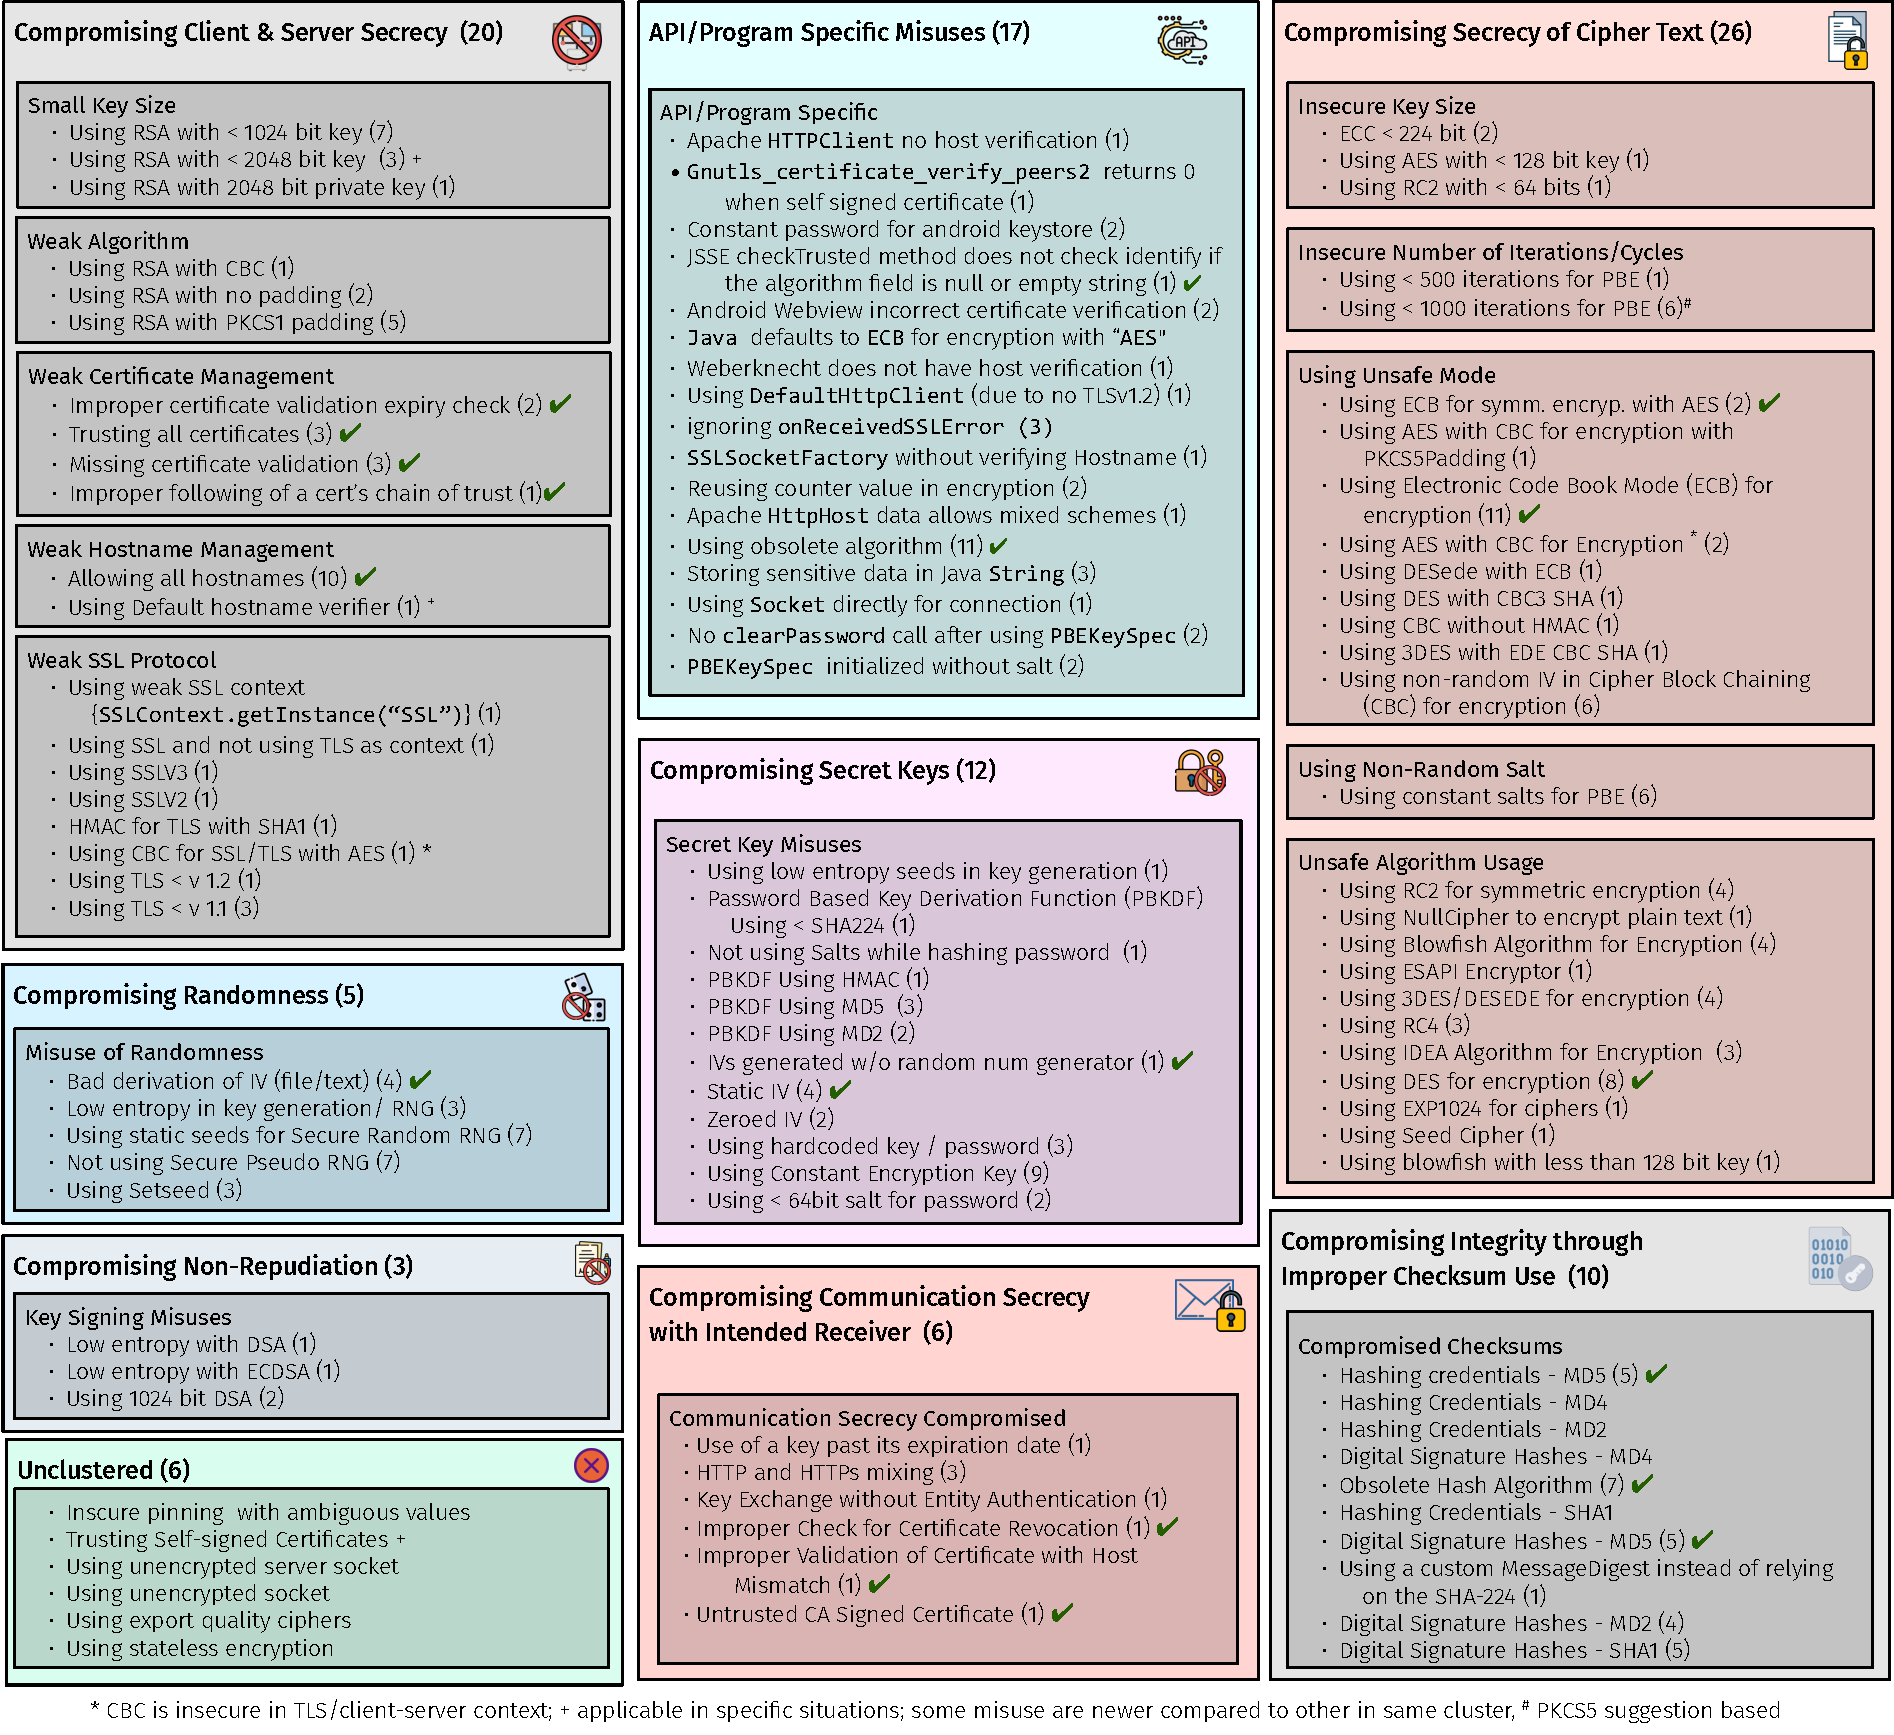
\includegraphics[width=0.96\linewidth]{figures/taxonomy.pdf}
	\vspace{-1.em}
    \caption{\small The orignal derived taxonomy of cryptographic misuses the extended taxnonmy is based on. ($n$) indicates misuse was present across $n$ artifacts.  A \checkmark indicates that the specific misuse case was instantiated with \tool's mutation operators for our evaluation.}
    \label{fig:taxonomy}
	
\end{figure*}
\begin{table*}
    
    \centering
    \caption{\small New misuse cases added to the taxonomy}
    \label{table:new_misuse}
    \begin{tabular}{ |c|c| } 
     \hline
    Misuse & \# Occurrences \\
    \hline
    Storing sensitive data in Java String & 5 \\
    \hline
    Key reuse in stream ciphers & 1 \\
    \hline
    Use of expired keys & 1 \\
    \hline
    No clearPassword call after using PBEKeySpec & 1 \\
    \hline
    Using AES-CTR & 1 \\
    \hline
    Weak algorithm for password-based encryption - PBKDF1 & 1 \\
    \hline
    HMAC for TLS with MD5 & 1 \\
    \hline
    Using RC5* & 1 \\
    \hline
    Using ARCFOUR & 1 \\
    \hline
    PBEWithMD5AndDES & 1 \\
    \hline
    Hashing Credentials - SHA-224 & 1 \\
    \hline
    Reusing IVs \& key pairs & 1 \\
    \hline
    Manually changing hostname verifier & 1 \\
     \hline
    \end{tabular}
    \end{table*}

In expanding MASC as a framework it was necessary to update the taxonomy to bring it up to date from when the original taxonomy was created in 2018. Above in Figure 2.2 the original taxonomy is shown and was the basis of this extension. Since the taxonomy is serving as expansion rather than a replacement the same methodology was used from its initial creation to extend it. This was done to ensure the taxonomy as a whole was consistent and one whole work rather than two different taxonomies. In order to locate academic and research papers related to Crypto-API misuse, it was first necessary to identify a set of search terms that would adequately narrow the search space. The authors of the original MASC paper had already identified a sufficiently narrowing set of search terms. 

These search terms were used, as well as combinations of these search terms, as a foundation in conducting our searches for academic and industrial papers published between 2019 and 2022 identifying Crypto-API misuse cases. This was also done to ensure the methods used to collect papers were consistent with the methods used in the original paper.  

With respect to academic papers, searches were conducted using the search terms laid out in the original work, as well as combinations of those terms on Google Scholar, IEEE Xplore \& ACM Digital Library as the primary search engines (these were also the engines used when creating the taxonomy for the original paper). In addition, each citing reference in each of the papers concerning Crypto-API misuse found through searching these databases and search engines was also looked at.  By doing this, it was possible to locate approximately 5-6 academic papers, concerning Crypto-API misuse, that were not readily visible through searches alone. This method helped expand the search domain for obtaining relevant academic papers.

For industrial sources, Google, Bing, and StackOverflow were relied upon for searching.  While it was possible to locate some relevant documents, they were few and far between compared to the academic papers that we uncovered.  In  an effort to ensure completeness of the search space,  when an industrial document relevant to Crypto-API misuse was located, the references it cited if any were also considered.

Additionally, a search was conducted through the Common Weakness Enumeration (CWE) from the MITRE Corporation \cite{MITRE}.  The CWE is a database of known hardware and software vulnerabilities, which are classified and categorized. Many crypto-detectors use CWE as a base for misuses that they detect.  Notably, it includes known weaknesses that involve software using an API (or Crypto API) in a manner contrary to its intended use.  A search was conducted using the CWE for new misuse cases not already identified in the original MASC Taxonomy or not already revealed in academic papers located from 2019 to 2022.  Unfortunately, the CWE did not contain any Crypto-API misuses that were not already contained in the MASC Taxonomy or based on our searches of academic papers from 2019 to 2022. 

To ensure that selected papers were only relevant to Crypto-API misuse in the MASC Taxonomy extension, the inclusion and exclusion criteria outlined in the original MASC paper was followed.  Specifically, to decide whether to consider a paper for further analysis, we used the inclusion criterion that the paper should discuss Crypto-API misuse or its detection. Exclusion criterion was used that the Crypto-API misuse described by the paper will be excluded if it does not relate to the Java programming environment or ecosystem, if the paper was published prior to 2019 or if the paper did not contain relevant information related to the subject of MASC.
    
In addition to these criteria, an additional exclusion criterion was included specifically with respect to the MASC Taxonomy extension.  That is, if a paper discussed Crypto-API-related misuses, but did not identify specific misuse cases in its text, the paper was added to the general list of sources.  However, these papers were not included in the final list of taxonomy sources from which misuse cases were extracted for the MASC Taxonomy extension. A complete list can be seen in Table \ref{table:new_papers}.

\begin{table*}
    
    \centering
    \tiny
    \caption{\small Papers added to the taxonomy}
    \label{table:new_papers}
    \begin{tabular}{ |c|c|c|c| } 
     \hline
    ID & Title & Year & Venue \\
    \hline
    37 & Ensuring correct cryptographic algorithm and provider usage at compile time \cite{Xing_Cheng_Dietl_2021} & 2021 & ACM \\
    \hline
    38 & Why Eve and Mallory Still Love Android: Revisiting TLS (In)Security in Android Applications \cite{oha+21} & 2021 & USENIX \\
    \hline
    39 & Towards HTTPS Everywhere on Android: We Are Not There Yet \cite{Possemato_Fratantonio} & 2020 & USENIX \\
    \hline
    40 & CRYPTOAPI-BENCH: A Comprehensive Benchmark on Java Cryptographic API Misuses \cite{Afrose_Rahaman_Yao_2019} & 2019 & IEEE \\
    \hline
    41 & CRYPTOREX: Large-scale Analysis of Cryptographic Misuse in IoT Devices \cite{ZCD+19} & 2019 & USENIX \\
    \hline
    42 & Negative Results on Mining Crypto-API Usage Rules in Android Apps \cite{GKL+19} & 2019 & IEEE \\
    \hline
    43 & Java Cryptography Uses in the Wild \cite{Hazhirpasand_Ghafari_Nierstrasz_2020} & 2020 & arXiv \\
    \hline
    44 & Python Crypto Misuses in the Wild \cite{Wickert_Baumgartner_Breitfelder_Mezini_2021} & 2021 & IEEE \\
    \hline
    45 & Understanding How to Use Static Analysis Tools for Detecting Cryptography Misuse in Software \cite{BDA+19} & 2019 & IEEE \\
    \hline
    46 & A Comparative Study of Misapplied Crypto in Android and iOS Applications \cite{Feichtner_2019} & 2019 & SECRYPT \\
    \hline
    47 & A Dataset of Parametric Cryptographic Misuses \cite{Wickert_Reif_Eichberg_Dodhy_Mezini_2019} & 2019 & IEEE \\
    \hline
    48 & CogniCryptGEN: generating code for the secure usage of crypto APIs \cite{Kruger_Ali_Bodden_2020} & 2020 & IEEE \\
    \hline
    49 & CryptoTutor: Teaching Secure Coding Practices through Misuse Pattern Detection \cite{Singleton_Zhao_Song_Siy_2020} & 2020 & ACM \\
    \hline
    50 & Using Graph Embeddings and Machine Learning to Detect Cryptography Misuse in Source Code \cite{Rodrigues_Braga_Dahab_2020} & 2020 & ICMLA \\
    \hline
    51 & Evaluation of Static Vulnerability Detection Tools with Java Cryptographic API Benchmarks \cite{Afrose_Xiao_Rahaman_Miller_Yao_2022} & 2022 & IEEE \\
    \hline
    52 & Automatic Detection of Java Cryptographic API Misuses: Are We There Yet? \cite{Zhang_Kabir_Xiao_Yao_Meng_2023} & 2023 & IEEE \\
    \hline
    53 & Hotfixing Misuses of Crypto APIs in Java Programs \cite{Newbury_Ali_Craik_2021} & 2021 & ACM \\
    \hline
    54 & CRYScanner: Finding cryptographic libraries misuse \cite{Choudhari_Guilley_Karray} & 2022 & IEEE \\
    \hline
    \end{tabular}
    \end{table*}

After compiling the master list of misuse sources, a misuse case extraction was performed. Two researchers independently identify and record misuse cases present within each of the sources. After this extraction process occurred, the two people  met and had what was termed an “agreement/disagreement meeting”, as described in the original paper, in order to discuss their findings with respect to our extractions.  This was done to ensure consistency across the different papers and ensure that each misuse case was found as well as confirmed. If the two members had any sort of disagreement over if something was a misuse case or not a third independent party was brought in to ensure correctness. 

Misuses were extracted and organized with the same methodology as the original paper. The same clusters were used that were designed for the original paper to organize each of the misuses into categories. The clusters were created based on two differentiating criteria: "(1) the security goal/property represented by the misuse case  (e.g., secrecy, integrity, non-repudiation) and (2) its level of abstraction within the communication/computing stack (e.g., confidentiality in general, or confidentiality with respect to SSL/TLS)"
    
In addition to this another misuse extraction was performed at a later date based on the misuses that were extracted. I went through each paper in the taxonomy and located each misuse that was listed for each of these new papers. This was done to confirm the work that had already been done but ensure that it was thorough. This step was meant to be redundant and ensure the correctness of the taxonomy but resulted in some disagreements of misuses within three of the sources and a disagreement with one of the new sources in the taxonomy as a whole. 

The approach for this additional step was for me to look at each individual paper. Based on the updated taxonomy that was produced I would go through the paper and look for each misuse that was specified to be contained within this paper. If the misuse was found it would be marked down and confirmed. If it was not found that misuse in the taxonomy would be flagged and would be brought up again with the original third party. Then if confirmed it would stay in the taxonomy if not it would be removed. Since the taxonomy is an extension I wanted to give extra cation to ensure not only correctness but consistency to ensure the taxonomy was one whole versus being two separate parts.
  
By the end of this process 13 new misuse cases were identified (see Table~\ref{table:new_misuse}) and added to the MASC Taxonomy. In addition, I was also able to further confirm many of the misuses that were already present in the taxonomy with the additional papers.



I believe that this is a solid basis for MASC as a whole and helped give ideas for expansion of operators to ensure that MASC is keeping up with the changing requirements. This taxonomy will likely have to be updated again in the future since security misuses come up frequently and the field is ever-changing. I feel that this taxonomy is a good representation of cryptographic misuses through 2022.

%--------------------------------------
\subsection{Extended Operators}
\label{ch2:sec:operators}
%--------------------------------------

When designing mutation operators I continued building them based on the trade-off of representing as many misuses cases as possible while also creating a number of operators that can still feasibly maintained. As the project grows this will continue to be a challenge. This is why it is important when operators were designed to make them as flexible to as many misuse cases as possible. This requires a lot of time and planning to ensure the design of the operators is maintainable. The other goal of operators as laid out in the original work is that they are not designed to exploit general soundiness limitations such as dynamic and implicit calls. This is important to ensure that the results that are found are actual flaws versus something that a tool cannot be reasonably expected to compute. The operators were designed to be expressive of multiple misuse cases to allow for more coverage. Design of operators is also guided by the threat model described previously. When an operator is designed which threat model it covers is considered as well. I felt there was a lot of room to expand upon the evasive developer (T3) so most of the new operators focus on this threat model.

The MASC framework consists of two main types of operators: flexible and restrictive operators. These two types are based on the common characteristics that were found amongst misuses of crypto-API. The restrictive operators are operators where a developer can only instantiate certain objects by providing values from a predefined set such the method Cipher.getInstance(<parameter>) only accepts predefined configuration values for the parameter in String form. While other crypto-APIs allow significant amount of customizability and extendability resulting in the flexible type of operators. For this work I exclusively focused on extending the restrictive operators.

Due to the nature of restrictive operators having more limitations it leaves plenty of room for expansion. In addition, since the taxonomy was expanded it was possible to utilize some of the ideas that already existed in the taxonomy as well as newly discovered misuse case. Since these operators have limitations, there are many possibilities for expanding the restrictive operators. For the extension of MASC we have focused heavily on expanding the number of restrictive operators as well as the functionality of some of the restrictive operators that already existed.

While expanding the operators there was also more of a focus placed on the (T3) cases. The initial paper was intentionally conservative with what was considered an evasive developer. This was due to the work being new and wanting to ensure that the operators were considered fair based on research conducted. After some time and further research I felt that it was possible to push further with this type of developer and after seeing further examples of evasive developers in real life cases. I wanted to ensure MASC is well-rounded when simulating different types of developers and provide the most use cases possible for crypto detectors.


\operator{13}{Iterative Method Chaining} Similar to in MASC \opnumber{5} (Method Chains) this operator implements method chaining to hide the value. Where this operator differs from \opnumber{5} is that it can take a value specified by the user and create that many method calls. The method calls are then chained in succession. Every method call will have a safe value until the final call which transforms the value into an unsafe value. This was created to test the limits of how far crypto detectors check method calls and can allow a user to determine where their fault point is. Just like \opnumber{5} this behavior would simulate a (T3) developer. An example can be seen in Appendix A at \ref{lst:iterativechaining}.

\operator{14}{Iterative Nested Conditionals} This operator shares some similarities with the idea behind \operator{13} but instead of using method calls based on the iteration value it creates nested conditionals based on the value. Within the if statement there is an unsafe value and in the else a safe value. The nested conditionals will always pass the unsafe value but like \operator{13} this operator tests how many nested conditionals a crypto detector can evaluate. An example can be seen in Appendix A at \ref{lst:iterativeconditionals}.

\operator{15}{Method Builder} This case takes method calls to build the String of a vulnerable call. The object class has methods that each contain a letter such as “D”, “E”, and “S”. Then it has a method that will add the letters together by calling each method and setting them equal to the variable in the class. This variable would now be "DES" and could be passed into an unsafe method. This operator also simulates (T3) behavior and is not something a developer would accidentally do. An example can be seen in Appendix A at \ref{lst:methodbuilder}.

\operator{16}{Object Sensitive} The operator creates two versions of a base object that has method calls to make a String either secure or unsecure. One object sets the variable to secure while the other sets itself to insecure. Then we set the object that is currently secure equal to the object that contains the insecure String. Then the originally secure object String is passed into the vulnerable API. This is done to test how well crypto detectors can handle object sensitivity. This was designed to give MASC more options for testing object sensitivity since this was an area that was originally lacking. The behavior also fits under our T3 developer. An example can be seen in Appendix A at  \ref{lst:ObjectSensitivity}.

\operator{17}{Build Variable} For this operator I converted an insecure String into a char array. Then when the vulnerability is passed into the API the char array is then converted back to a String during the method call. This would fall under the (T1, T2) developer. This is because a developer could be doing some form of String manipulation that requires converting a String to a char array and then passing that into the method call. An example can be seen in Appendix A at  \ref{lst:buildvariable}.

\operator{18}{Substring} The idea behind this case is a user pulling the misuse out of a substring. In this case we took something like “HelloWorldDES” and passed the substring “DES” into the vulnerable API. Once again this is a (T1, T2) developer since they might pull something out of String and pass it in not knowing that it is vulnerable. Since it is not being passed in simply as a String if the crypto detector does not process the change this is easily a misuse that could slip by. An example can be seen in Appendix A at  \ref{lst:substring}.

\operator{19}{Static Keystore} This operator is designed to handle static bytes being passed in insecure ways. For example, if a developer attempted to pass static bytes that are stored in a variable into Android Keystore since this is considered unsecure behavior. This would emulate a T1 developer since this is a very easy mistake to make if someone is unaware of the rules associated with crypto API and vulnerabilities. An example can be seen in Appendix A at  \ref{lst:statickeystore}.



%--------------------------------------
\subsection{Threat Based Mutation Scopes}
\label{ch2:sec:scopes}
%--------------------------------------

The mutation scopes are designed to emulate the three types of developers described in the threat model. The scopes try to closely simulate placements of vulnerable code for the benign (T1, T2) and evasive developers:

The main scope creates base case mutations and generates simple Java files to be tested. This is used mainly to determine if a crypto-detector is even capable of detecting misuses in the most plain cases. These mutants are seeded in simple Java or Android templates at the beginning of the main method. This ensures that the mutants are found and analyzed. This is meant to simulate the behavior of a benign (T1 and T2) developer.

The exhaustive scope looks at seeding mutations in every possible location such as class definitions, conditional segments, method bodies and anonymous inner class object declarations. Note that it is seeded in places that ensure the app is still compilable. Typically, this is used with a single misuse that is known to be detected by the operator and is used to determine how thorough the crypto-detectors when analyzing files. This scope is meant to analyze a T3 developer they may hide misuses in places that one would not normally expect misuses to appear.

The similarity scope seeds mutants in places where a similar security API is already in use. It emulates taking possibly secure uses and making them insecure while not overwriting the previous code. This emulates where the benign developers (T1 and T2) would potentially place misuses and is meant to test how well the crypto-detectors analyze realistic areas misuses might appear. 
